\documentclass[11pt]{article}
\usepackage[margin=25mm]{geometry}
\usepackage{graphicx,amsmath,booktabs,pdfpages}
\begin{document}
\section*{Numerical experiment: raw Hyperplane Sweep versus GW}
We use all 71 canonical G-set graphs, with one fixed archived EVA embedding per graph and 16 shared initial GW normals. At each of 100 subsequent steps, the two methods receive the same fresh Gaussian draw. GW uses its normalized direction as a new independent hyperplane; Hyperplane Sweep projects the draw perpendicular to its current incumbent and searches the entire resulting semicircle. Both retain their best cut so far. No EVA, clustering or discrete local-search refinement is performed.
For graph \(g\), restart \(s\), method \(m\), and step \(t\), define \(B_{gms}(t)\) as the best cut found so far and \(\bar C_g\) as the mean initial GW cut. The plotted gain is
\[
G_m(t)=\frac{100}{71\cdot16}\sum_{g,s}
 \frac{B_{gms}(t)-B_{gms}(0)}{\bar C_g}.
\]

After 100 steps, repeated GW improved by 2.4110\% and the sweep by 4.2389\%.
The difference is +1.8279 percentage points (descriptive graph-bootstrap 95\% interval [1.5079, 2.1602]).
The sweep wins/ties/loses on 69/2/0 graphs by mean final cut.
All 229472 candidate scores were independently rescored using the original signed graph edges.
\begin{center}
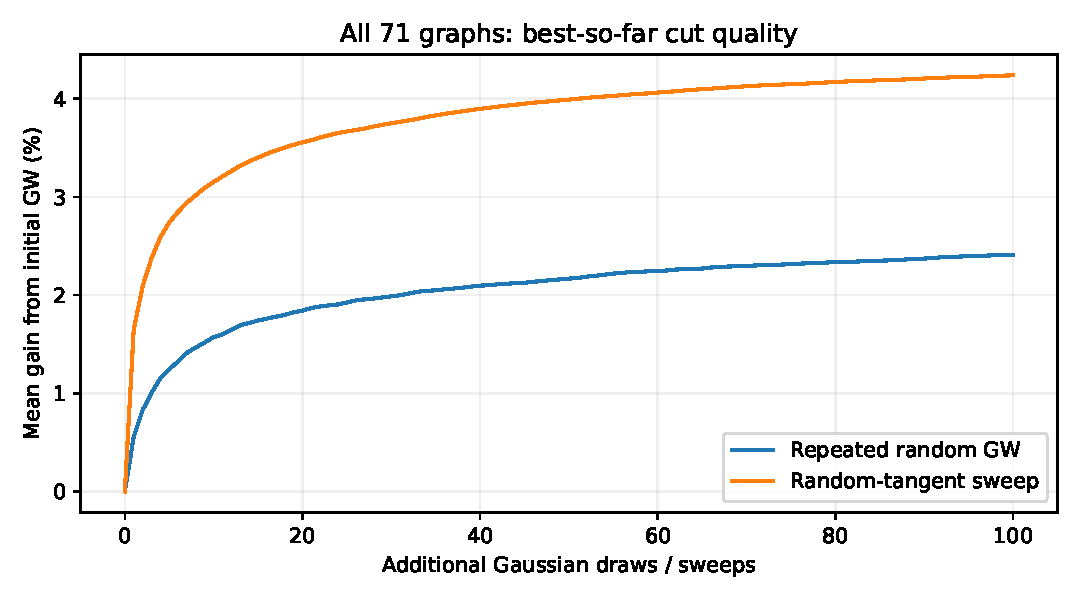
\includegraphics[width=.98\linewidth]{convergence.pdf}
\end{center}
\clearpage
\section*{Computational cost and variation among graphs}
Equal numbers of Gaussian draws do not imply equal computational work: a sweep examines many event intervals, while GW samples just one partition. The time plot averages measured cumulative algorithm times and is not an equal-time experiment. Compilation, random number generation, archive I/O and external verification are excluded. The following pages show individual learning curves for every graph. These are empirical results, not a certificate of global optimality.
\begin{center}
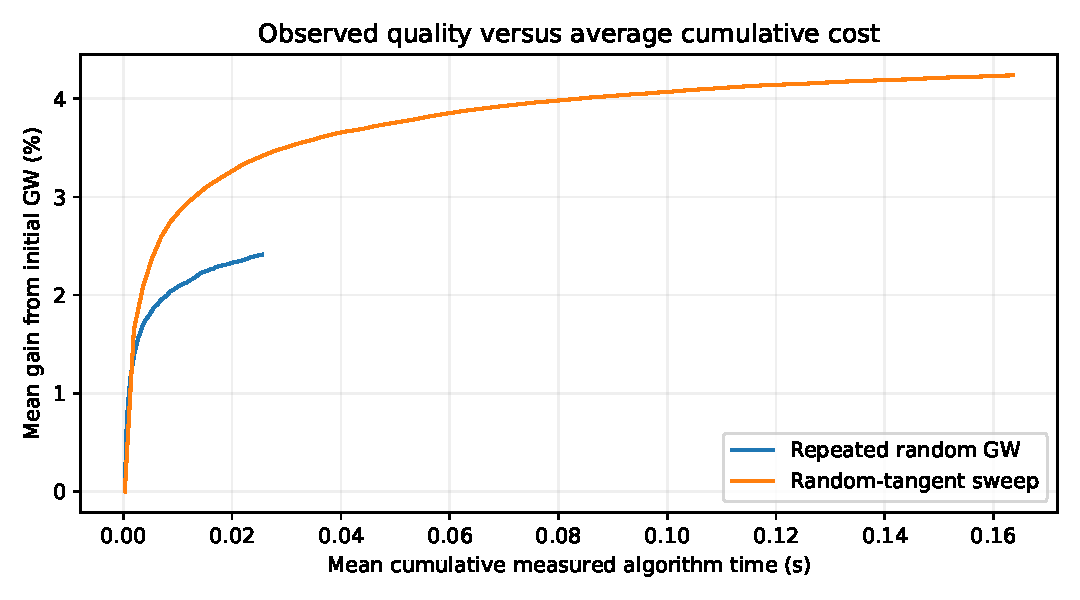
\includegraphics[width=.90\linewidth]{time_quality.pdf}

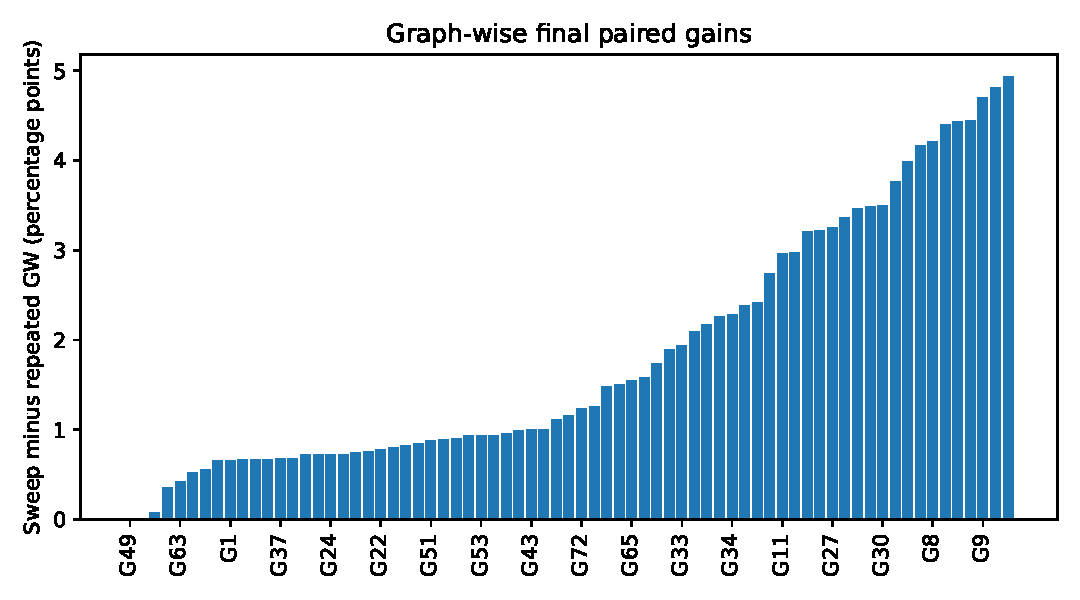
\includegraphics[width=.90\linewidth]{graph_gains.pdf}
\end{center}
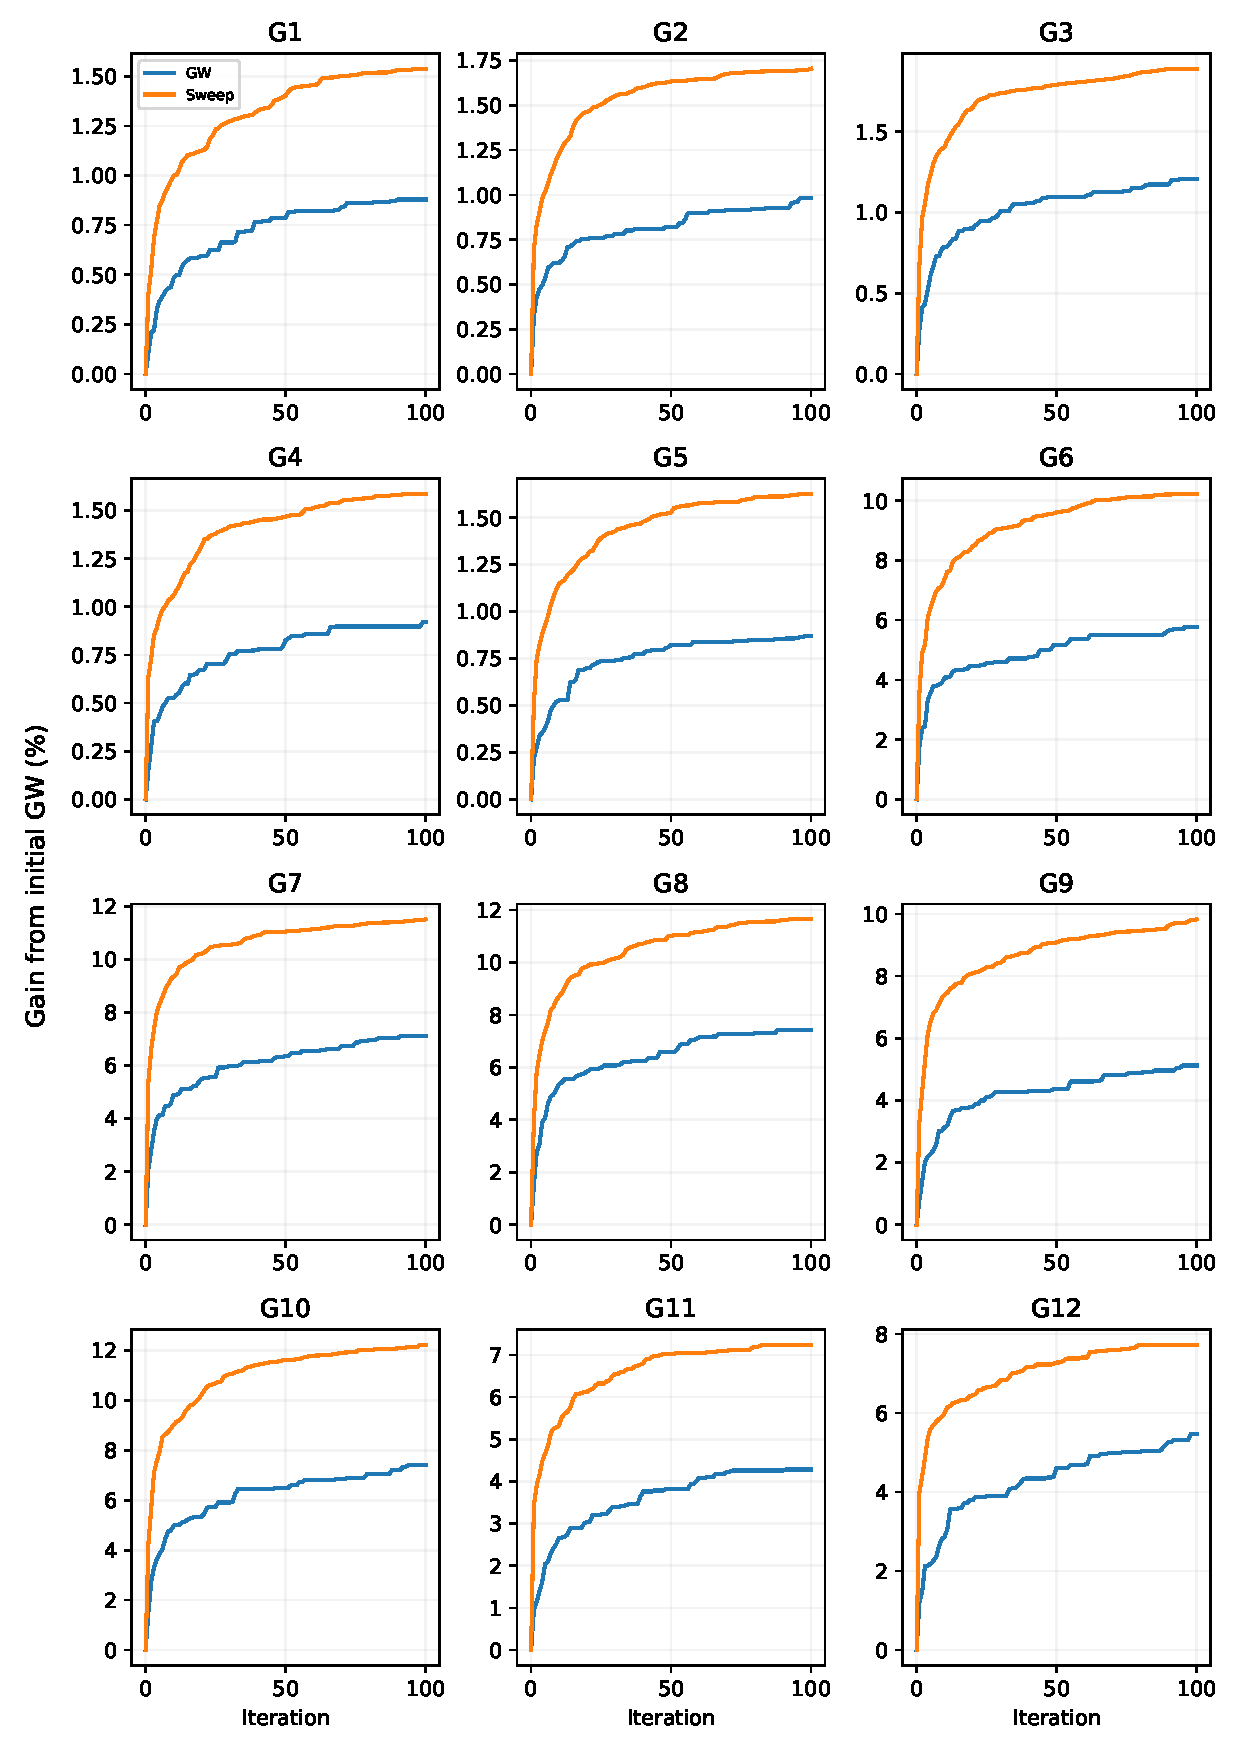
\includepdf[pages=-]{all_71_curves.pdf}
\end{document}
